\documentclass[]{article}

\usepackage{graphicx,type1cm,eso-pic,color}
\usepackage[spanish]{babel} %%%% for


\makeatletter
          \AddToShipoutPicture{
            \setlength{\@tempdimb}{.95\paperwidth}
            \setlength{\@tempdimc}{.5\paperheight}
            \setlength{\unitlength}{1pt}
            \put(\strip@pt\@tempdimb,\strip@pt\@tempdimc){
        \makebox(0,0){\rotatebox{-90}{\textcolor[gray]{0.90}
        {\fontsize{.65cm}{.5cm}\selectfont{\rm Dae-Jin Lee}}}}
            }
        }
          \AddToShipoutPicture{
            \setlength{\@tempdimb}{.50\paperwidth}
            \setlength{\@tempdimc}{.95\paperheight}
            \setlength{\unitlength}{1pt}
            \put(\strip@pt\@tempdimb,\strip@pt\@tempdimc){
        \makebox(0,0){\rotatebox{0}{\textcolor[gray]{0.90}
        {\fontsize{.5cm}{.5cm}\selectfont{\rm Curso de Estad\'istica b\'asica para Data Scientist  - @datahack}}}}
            }
        }
\makeatother

\def\tightlist{}

\usepackage{lmodern}
\usepackage{amssymb,amsmath}
\usepackage{ifxetex,ifluatex}
\usepackage{fixltx2e} % provides \textsubscript
\ifnum 0\ifxetex 1\fi\ifluatex 1\fi=0 % if pdftex
  \usepackage[T1]{fontenc}
  \usepackage[utf8]{inputenc}
\else % if luatex or xelatex
  \ifxetex
    \usepackage{mathspec}
    \usepackage{xltxtra,xunicode}
  \else
    \usepackage{fontspec}
  \fi
  \defaultfontfeatures{Mapping=tex-text,Scale=MatchLowercase}
  \newcommand{\euro}{???}
\fi
% use upquote if available, for straight quotes in verbatim environments
\IfFileExists{upquote.sty}{\usepackage{upquote}}{}
% use microtype if available
\IfFileExists{microtype.sty}{%
\usepackage{microtype}
\UseMicrotypeSet[protrusion]{basicmath} % disable protrusion for tt fonts
}{}
\usepackage{color}
\usepackage{fancyvrb}
\newcommand{\VerbBar}{|}
\newcommand{\VERB}{\Verb[commandchars=\\\{\}]}
\DefineVerbatimEnvironment{Highlighting}{Verbatim}{commandchars=\\\{\}}
% Add ',fontsize=\small' for more characters per line
\usepackage{framed}
\definecolor{shadecolor}{RGB}{248,248,248}
\newenvironment{Shaded}{\begin{snugshade}}{\end{snugshade}}
\newcommand{\KeywordTok}[1]{\textcolor[rgb]{0.13,0.29,0.53}{\textbf{{#1}}}}
\newcommand{\DataTypeTok}[1]{\textcolor[rgb]{0.13,0.29,0.53}{{#1}}}
\newcommand{\DecValTok}[1]{\textcolor[rgb]{0.00,0.00,0.81}{{#1}}}
\newcommand{\BaseNTok}[1]{\textcolor[rgb]{0.00,0.00,0.81}{{#1}}}
\newcommand{\FloatTok}[1]{\textcolor[rgb]{0.00,0.00,0.81}{{#1}}}
\newcommand{\ConstantTok}[1]{\textcolor[rgb]{0.00,0.00,0.00}{{#1}}}
\newcommand{\CharTok}[1]{\textcolor[rgb]{0.31,0.60,0.02}{{#1}}}
\newcommand{\SpecialCharTok}[1]{\textcolor[rgb]{0.00,0.00,0.00}{{#1}}}
\newcommand{\StringTok}[1]{\textcolor[rgb]{0.31,0.60,0.02}{{#1}}}
\newcommand{\VerbatimStringTok}[1]{\textcolor[rgb]{0.31,0.60,0.02}{{#1}}}
\newcommand{\SpecialStringTok}[1]{\textcolor[rgb]{0.31,0.60,0.02}{{#1}}}
\newcommand{\ImportTok}[1]{{#1}}
\newcommand{\CommentTok}[1]{\textcolor[rgb]{0.56,0.35,0.01}{\textit{{#1}}}}
\newcommand{\DocumentationTok}[1]{\textcolor[rgb]{0.56,0.35,0.01}{\textbf{\textit{{#1}}}}}
\newcommand{\AnnotationTok}[1]{\textcolor[rgb]{0.56,0.35,0.01}{\textbf{\textit{{#1}}}}}
\newcommand{\CommentVarTok}[1]{\textcolor[rgb]{0.56,0.35,0.01}{\textbf{\textit{{#1}}}}}
\newcommand{\OtherTok}[1]{\textcolor[rgb]{0.56,0.35,0.01}{{#1}}}
\newcommand{\FunctionTok}[1]{\textcolor[rgb]{0.00,0.00,0.00}{{#1}}}
\newcommand{\VariableTok}[1]{\textcolor[rgb]{0.00,0.00,0.00}{{#1}}}
\newcommand{\ControlFlowTok}[1]{\textcolor[rgb]{0.13,0.29,0.53}{\textbf{{#1}}}}
\newcommand{\OperatorTok}[1]{\textcolor[rgb]{0.81,0.36,0.00}{\textbf{{#1}}}}
\newcommand{\BuiltInTok}[1]{{#1}}
\newcommand{\ExtensionTok}[1]{{#1}}
\newcommand{\PreprocessorTok}[1]{\textcolor[rgb]{0.56,0.35,0.01}{\textit{{#1}}}}
\newcommand{\AttributeTok}[1]{\textcolor[rgb]{0.77,0.63,0.00}{{#1}}}
\newcommand{\RegionMarkerTok}[1]{{#1}}
\newcommand{\InformationTok}[1]{\textcolor[rgb]{0.56,0.35,0.01}{\textbf{\textit{{#1}}}}}
\newcommand{\WarningTok}[1]{\textcolor[rgb]{0.56,0.35,0.01}{\textbf{\textit{{#1}}}}}
\newcommand{\AlertTok}[1]{\textcolor[rgb]{0.94,0.16,0.16}{{#1}}}
\newcommand{\ErrorTok}[1]{\textcolor[rgb]{0.64,0.00,0.00}{\textbf{{#1}}}}
\newcommand{\NormalTok}[1]{{#1}}
\usepackage{longtable,booktabs}
\usepackage{graphicx}
\makeatletter
\def\maxwidth{\ifdim\Gin@nat@width>\linewidth\linewidth\else\Gin@nat@width\fi}
\def\maxheight{\ifdim\Gin@nat@height>\textheight\textheight\else\Gin@nat@height\fi}
\makeatother
% Scale images if necessary, so that they will not overflow the page
% margins by default, and it is still possible to overwrite the defaults
% using explicit options in \includegraphics[width, height, ...]{}
\setkeys{Gin}{width=\maxwidth,height=\maxheight,keepaspectratio}
\ifxetex
  \usepackage[setpagesize=false, % page size defined by xetex
              unicode=false, % unicode breaks when used with xetex
              xetex]{hyperref}
\else
  \usepackage[unicode=true]{hyperref}
\fi
\hypersetup{breaklinks=true,
            bookmarks=true,
            pdfauthor={Dae-Jin Lee \textless{} lee.daejin@gmail.com \textgreater{}},
            pdftitle={Curso de Estadística básica para Data Scientists},
            colorlinks=true,
            citecolor=blue,
            urlcolor=blue,
            linkcolor=magenta,
            pdfborder={0 0 0}}
\urlstyle{same}  % don't use monospace font for urls
\setlength{\parindent}{0pt}
\setlength{\parskip}{6pt plus 2pt minus 1pt}
\setlength{\emergencystretch}{3em}  % prevent overfull lines
\setcounter{secnumdepth}{5}

\title{\textbf{Curso de Estadística básica para Data Scientists}}
\author{Dae-Jin Lee \textless{}
\href{mailto:lee.daejin@gmail.com}{\nolinkurl{lee.daejin@gmail.com}}
\textgreater{}}
\date{TEMA 6. Modelos lineales}

\usepackage{amsfonts}
\usepackage{amsmath}
\usepackage{amssymb}
\usepackage{natbib}
%\usepackage[T1]{fontenc}
\usepackage{latexsym}
\usepackage{graphicx}
\usepackage{caption}
\usepackage{subcaption}
\usepackage{color}
\usepackage{algorithm2e}
%%
%     Definitions
%
\newcommand{\tri}{\bigtriangleup}
\newcommand{\Xp}{X^\prime}
\newcommand{\E}{\mbox{E}}
\newcommand{\Hh}{\mbox{H}}
\newcommand{\V}{\mbox{Var}}
\newcommand{\tr}{\mbox{tr}}
\newcommand{\CV}{\mbox{CV}}
\newcommand{\GCV}{\mbox{GCV}}
\newcommand{\AIC}{\mbox{AIC}}
\newcommand{\ph}{\phantom{0}}
\newcommand{\half}{\mbox{${1\over2}$}}
\newcommand{\bfzero}{\boldsymbol{0}}
\newcommand{\bfone}{\boldsymbol{1}}

\newcommand{\bfa}{\boldsymbol{a}}
\newcommand{\bfb}{\boldsymbol{b}}
\newcommand{\bfe}{\boldsymbol{e}}
\newcommand{\bff}{\boldsymbol{f}}
\newcommand{\bfg}{\boldsymbol{g}}
\newcommand{\bfs}{\boldsymbol{s}}
\newcommand{\bfu}{\boldsymbol{u}}
\newcommand{\bfx}{\boldsymbol{x}}
\newcommand{\bfy}{\boldsymbol{y}}
\newcommand{\bfz}{\boldsymbol{z}}

\newcommand{\bfA}{\boldsymbol{A}}
\newcommand{\bfB}{\boldsymbol{B}}
\newcommand{\bfC}{\boldsymbol{C}}
\newcommand{\bfD}{\boldsymbol{D}}
\newcommand{\bfF}{\boldsymbol{F}}
\newcommand{\bfG}{\boldsymbol{G}}
\newcommand{\bfH}{\boldsymbol{H}}
\newcommand{\bfI}{\boldsymbol{I}}
\newcommand{\bfM}{\boldsymbol{M}}
\newcommand{\bfP}{\boldsymbol{P}}
\newcommand{\bfQ}{\boldsymbol{Q}}
\newcommand{\bfR}{\boldsymbol{R}}
\newcommand{\bfS}{\boldsymbol{S}}
\newcommand{\bfT}{\boldsymbol{T}}
\newcommand{\bfU}{\boldsymbol{U}}
\newcommand{\bfV}{\boldsymbol{V}}
\newcommand{\bfW}{\boldsymbol{W}}
\newcommand{\bfX}{\boldsymbol{X}}
\newcommand{\bfY}{\boldsymbol{Y}}
\newcommand{\bfZ}{\boldsymbol{Z}}


\newcommand{\bfalpha}{\boldsymbol{\alpha}}
\newcommand{\bfbeta}{\boldsymbol{\beta}}
\newcommand{\bfepsilon}{\boldsymbol{\epsilon}}
\newcommand{\bfgamma}{\boldsymbol{\gamma}}
\newcommand{\bfGamma}{\boldsymbol{\Gamma}}
\newcommand{\bfmu}{\boldsymbol{\mu}}
\newcommand{\bfeta}{\boldsymbol{\eta}}
\newcommand{\bfrho}{\boldsymbol{\rho}}
\newcommand{\bftheta}{\boldsymbol{\theta}}
\newcommand{\bfxi}{\boldsymbol{\xi}}
\newcommand{\bftau}{\boldsymbol{\tau}}
\newcommand{\bflambda}{\boldsymbol{\lambda}}
\newcommand{\bfsigma}{\boldsymbol{\sigma}}
\newcommand{\bfLambda}{\boldsymbol{\Lambda}}
\newcommand{\bfSigma}{\boldsymbol{\Sigma}}

\renewcommand{\theequation}{\thesection.\arabic{equation}}
\numberwithin{equation}{section}

\begin{document}
\maketitle

{
\hypersetup{linkcolor=black}
\setcounter{tocdepth}{2}
\tableofcontents
}
\newpage

\href{https://idaejin.github.io/bcam-courses/R/datahack/}{Regresar a la
página principal}

\section{\texorpdfstring{Modelos lineales en
\texttt{R}}{Modelos lineales en R}}\label{modelos-lineales-en-r}

\subsection{Regresión lineal simple}\label{regresion-lineal-simple}

\begin{itemize}
\item
  La regresión es un método estadístico utilizado para predecir el valor
  de una variable de respuesta basada en los valores de un conjunto de
  variables explicativas.
\item
  Una forma muy general para el modelo sería
\end{itemize}

\[
      y = f(x_1,x_2,...,x_p) + \epsilon,
\]

donde \(f\) es una función desconocida y \(\epsilon\) es el error en
esta representación. Dado que usualmente no tenemos suficientes datos
para tratar de estimar \(f\) directamente (\emph{problema inverso}),
normalmente tenemos que suponer que tiene alguna forma restringida.

\begin{itemize}
\item
  Cualquier modelo estadístico intenta aproximar la variable de
  respuesta o variable dependiente \(y\) como una función matemática de
  las variables explicativas o regresores \(X\) (también llamadas
  covariables o variables independientes).
\item
  La forma más sencilla y más común es la \textbf{regresión lineal}
\end{itemize}

\[
    y = \beta_0 + \beta_1 x_1 + \beta_2 x_z + \epsilon,
\] donde \(\beta_i\) \(i=0,1,2\) son parametros \emph{desconocidos}.
\(\beta_0\) se llama el intercepto. Por lo tanto, el problema se reduce
a la estimación de cuatro valores en lugar de la complicada infinita
dimensión \(f\).

\begin{itemize}
\tightlist
\item
  Un modelo lineal simple con una sola variable explicativa se define
  como:
\end{itemize}

\[
         \hat{y} = \beta_0 + \beta_1 x
\]

donde \(\hat y\) son los valores ajustados para \(\beta_0\) (intercepto)
y \(\beta_1\) (pendiente). Entonces para un \(x_i\) dado obtenemos un
\(\hat{y}_i\) que se aproxima a \(y_i\)

Supongamos el siguiente ejemplo simulado (con \(p=1\)):

\begin{Shaded}
\begin{Highlighting}[]
\KeywordTok{set.seed}\NormalTok{(}\DecValTok{1}\NormalTok{)}
\NormalTok{n <-}\StringTok{ }\DecValTok{50} 

\NormalTok{x <-}\StringTok{ }\KeywordTok{seq}\NormalTok{(}\DecValTok{1}\NormalTok{,n)}
 \NormalTok{beta0 <-}\StringTok{ }\DecValTok{15}
 \NormalTok{beta1 <-}\StringTok{ }\FloatTok{0.5}

\NormalTok{sigma <-}\StringTok{ }\DecValTok{3} \CommentTok{# standar deviation of the errors}
\NormalTok{eps <-}\StringTok{ }\KeywordTok{rnorm}\NormalTok{(n,}\DataTypeTok{mean=}\DecValTok{0}\NormalTok{,}\DataTypeTok{sd=}\DecValTok{3}\NormalTok{) }\CommentTok{# generate gaussian random errors}

\CommentTok{# Generate random data}
 \NormalTok{y <-}\StringTok{ }\NormalTok{beta0 +}\StringTok{ }\NormalTok{beta1*x  +}\StringTok{  }\NormalTok{eps}
\end{Highlighting}
\end{Shaded}

Plot de los datos

\begin{Shaded}
\begin{Highlighting}[]
\KeywordTok{plot}\NormalTok{(x,y,}\DataTypeTok{ylim =} \KeywordTok{c}\NormalTok{(}\DecValTok{8}\NormalTok{,}\DecValTok{45}\NormalTok{), }\DataTypeTok{cex=}\FloatTok{1.3}\NormalTok{, }\DataTypeTok{xlab =} \StringTok{"x"}\NormalTok{, }\DataTypeTok{ylab=}\StringTok{"y"}\NormalTok{,}\DataTypeTok{pch=}\DecValTok{19}\NormalTok{)}
\end{Highlighting}
\end{Shaded}

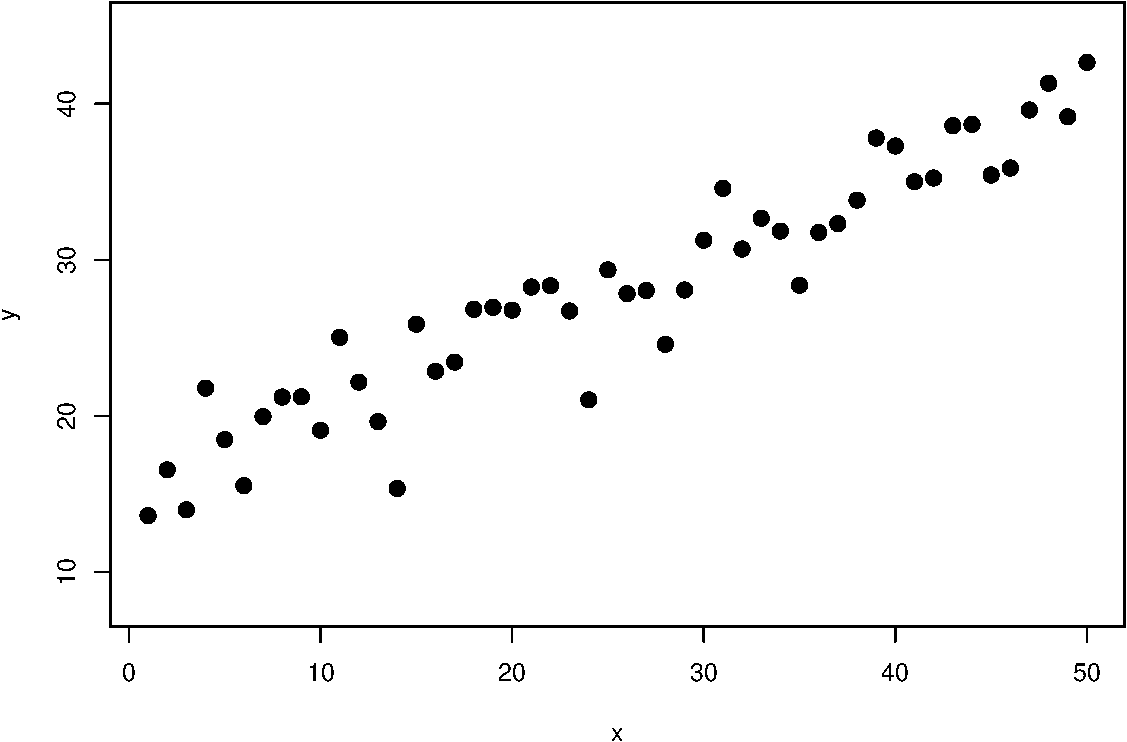
\includegraphics{tema6_files/figure-latex/unnamed-chunk-2-1.pdf}
Procedimiento matemático para encontrar la curva que mejor se ajuste a
un conjunto de puntos dado, resulta de minimizar la suma de los
cuadrados de los residuos de los puntos de la línea ajustada.
Ilustración del ajuste de mínimos cuadrados

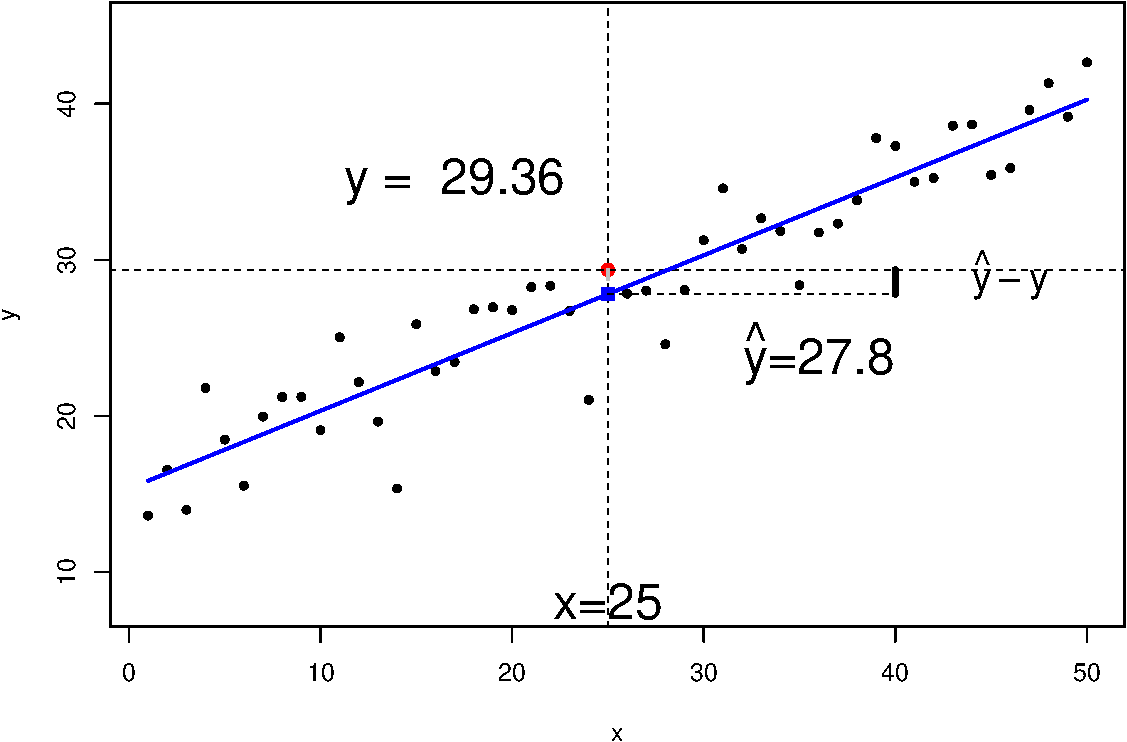
\includegraphics{tema6_files/figure-latex/unnamed-chunk-3-1.pdf}

Por ejemplo, en el conjunto de datos \texttt{faithful}, contiene datos
de ejemplo de dos variables aleatorias denominadas \texttt{waiting} y
\texttt{eruptions}. La variable \texttt{waiting} indica el tiempo de
espera hasta las próximas erupciones, y\texttt{eruptions} denota la
duración.

\begin{Shaded}
\begin{Highlighting}[]
\KeywordTok{plot}\NormalTok{(eruptions~waiting,}\DataTypeTok{data=}\NormalTok{faithful)}
\end{Highlighting}
\end{Shaded}

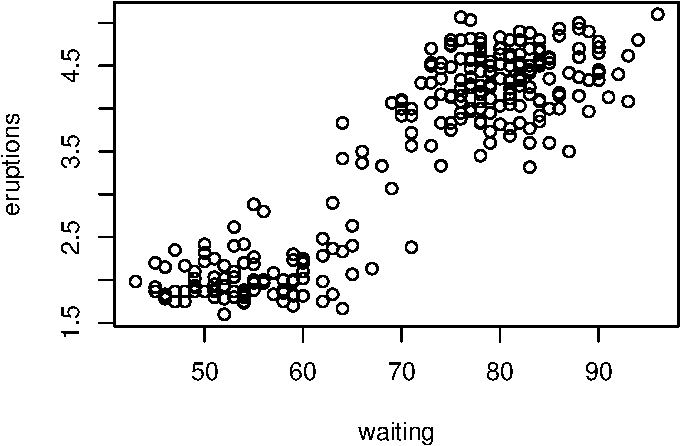
\includegraphics{tema6_files/figure-latex/unnamed-chunk-4-1.pdf}

El modelo lineal viene dado por:

\[
Eruptions = \beta_0 + \beta_1*Waiting + \epsilon
\]

Si seleccionamos los parámetros \(\beta_0\) y \(\beta_1\) en el modelo
de regresión lineal simple para minimizar la suma de cuadrados del
término de error \(\epsilon\). Supongamos que para el conjunto de datos
\texttt{faithful}, pretendemos estimar la siguiente duración de la
erupción si el tiempo de espera desde la última erupción ha sido de 80
minutos. Aplicamos la función \texttt{lm} a una fórmula que describe la
variable erupciones por la variable waiting, y guardamos el modelo de
regresión lineal en una nueva variable \texttt{eruption.lm}.

\begin{Shaded}
\begin{Highlighting}[]
\KeywordTok{data}\NormalTok{(}\StringTok{"faithful"}\NormalTok{)}
\NormalTok{eruption.lm <-}\StringTok{ }\KeywordTok{lm}\NormalTok{(eruptions~waiting,}\DataTypeTok{data=}\NormalTok{faithful)}
\end{Highlighting}
\end{Shaded}

Extraemos los parámetros de la ecuación de regresión estimada con la
función de coeficientes.

\begin{Shaded}
\begin{Highlighting}[]
\NormalTok{coeffs <-}\StringTok{ }\KeywordTok{coefficients}\NormalTok{(eruption.lm); coeffs }
\end{Highlighting}
\end{Shaded}

\begin{verbatim}
## (Intercept)     waiting 
## -1.87401599  0.07562795
\end{verbatim}

Ahora ajustamos la duración de la erupción usando la ecuación de
regresión estimada.

\begin{Shaded}
\begin{Highlighting}[]
\NormalTok{waiting =}\StringTok{ }\DecValTok{80}           \CommentTok{# the waiting time }
\NormalTok{duration =}\StringTok{ }\NormalTok{coeffs[}\DecValTok{1}\NormalTok{] +}\StringTok{ }\NormalTok{coeffs[}\DecValTok{2}\NormalTok{]*waiting }
\NormalTok{duration }
\end{Highlighting}
\end{Shaded}

\begin{verbatim}
## (Intercept) 
##     4.17622
\end{verbatim}

En base al modelo de regresión lineal simple, si el tiempo de espera
desde la última erupción ha sido de 80 minutos, esperamos que los
próximos minutos de duración 4.1762198.

Podemos incluir el valor de \texttt{waiting=80} en \texttt{newdata} como
un \texttt{data.frame}

\begin{Shaded}
\begin{Highlighting}[]
\NormalTok{newdata =}\StringTok{ }\KeywordTok{data.frame}\NormalTok{(}\DataTypeTok{waiting=}\DecValTok{80}\NormalTok{) }\CommentTok{# wrap the parameter }
\end{Highlighting}
\end{Shaded}

Y aplicar la función \texttt{predict} a modelo \texttt{eruption.lm} con
\texttt{newdata}.

\begin{Shaded}
\begin{Highlighting}[]
\KeywordTok{predict}\NormalTok{(eruption.lm, newdata)    }\CommentTok{# apply predict }
\end{Highlighting}
\end{Shaded}

\begin{verbatim}
##       1 
## 4.17622
\end{verbatim}

Podemos calcular directamente las cantidades de interés, es decir, la
solución de mínimos cuadrados ordinarios consiste en:

\[
\min_{\beta_0,\beta_1} = \sum_{i=1}^{n} (y_i - \hat{y}_i)^2  
\]

Por tanto
\(\hat{\beta}_1 = \frac{\sum_{i=1}^{n}x_iy_i}{\sum_{i=1}^n x_i^2}\) and
\(\hat{\beta}_0 = \bar{y} - \hat{\beta}_1\bar{x}\)

En forma de matricial, con \(X=[1:x_1:...:x_p]\)

\[
\hat{\beta}  = (X^\prime X)^{-1} X^\prime
\]

donde \(\hat{\beta} = (\hat{\beta}_0,\hat{\beta}_1)\)

\subsection{\texorpdfstring{Definir modelos en
\texttt{R}}{Definir modelos en R}}\label{definir-modelos-en-r}

Para completar una regresión lineal usando \texttt{R} es necesario
primero entender la sintaxis para definir modelos.

\begin{longtable}[]{@{}ccc@{}}
\toprule
\begin{minipage}[b]{0.14\columnwidth}\centering\strut
Syntax\strut
\end{minipage} & \begin{minipage}[b]{0.29\columnwidth}\centering\strut
Model\strut
\end{minipage} & \begin{minipage}[b]{0.48\columnwidth}\centering\strut
Comments\strut
\end{minipage}\tabularnewline
\midrule
\endhead
\begin{minipage}[t]{0.14\columnwidth}\centering\strut
\texttt{y\ \textasciitilde{}\ x}\strut
\end{minipage} & \begin{minipage}[t]{0.29\columnwidth}\centering\strut
\(y = \beta_0+\beta_1x\)\strut
\end{minipage} & \begin{minipage}[t]{0.48\columnwidth}\centering\strut
Linea recta con intercepto\strut
\end{minipage}\tabularnewline
\begin{minipage}[t]{0.14\columnwidth}\centering\strut
\texttt{y\ \textasciitilde{}\ -1\ +\ x}\strut
\end{minipage} & \begin{minipage}[t]{0.29\columnwidth}\centering\strut
\(y = \beta_1x\)\strut
\end{minipage} & \begin{minipage}[t]{0.48\columnwidth}\centering\strut
Linea recta sin intercepto, i.e.~la recta pasa por (0,0)\strut
\end{minipage}\tabularnewline
\begin{minipage}[t]{0.14\columnwidth}\centering\strut
\texttt{y\ \textasciitilde{}\ x\ +\ I(x\^{}2)}\strut
\end{minipage} & \begin{minipage}[t]{0.29\columnwidth}\centering\strut
\(y = \beta_0+\beta_1x+\beta_2x^2\)\strut
\end{minipage} & \begin{minipage}[t]{0.48\columnwidth}\centering\strut
Modelo polinomial; \texttt{I()} permite incluir símbolos
matemáticos\strut
\end{minipage}\tabularnewline
\begin{minipage}[t]{0.14\columnwidth}\centering\strut
\texttt{y\ \textasciitilde{}\ x\ +\ z}\strut
\end{minipage} & \begin{minipage}[t]{0.29\columnwidth}\centering\strut
\(y = \beta_0+\beta_1x+\beta_2z\)\strut
\end{minipage} & \begin{minipage}[t]{0.48\columnwidth}\centering\strut
Model de regresión múltiple\strut
\end{minipage}\tabularnewline
\begin{minipage}[t]{0.14\columnwidth}\centering\strut
\texttt{y\ \textasciitilde{}\ x:z}\strut
\end{minipage} & \begin{minipage}[t]{0.29\columnwidth}\centering\strut
\(y = \beta_0+\beta_1xz\)\strut
\end{minipage} & \begin{minipage}[t]{0.48\columnwidth}\centering\strut
Modelo con interacción entre \(x\) y \(z\)\strut
\end{minipage}\tabularnewline
\begin{minipage}[t]{0.14\columnwidth}\centering\strut
\texttt{y\ \textasciitilde{}\ x*z}\strut
\end{minipage} & \begin{minipage}[t]{0.29\columnwidth}\centering\strut
\(y = \beta_0+\beta_1x+\beta_2z+\beta_3xz\)\strut
\end{minipage} & \begin{minipage}[t]{0.48\columnwidth}\centering\strut
Equivale a \texttt{y\textasciitilde{}x+z+x:z}\strut
\end{minipage}\tabularnewline
\bottomrule
\end{longtable}

En \texttt{R} la función \texttt{model.matrix} permite crear la matriz
de diseño \(X\).

\begin{Shaded}
\begin{Highlighting}[]
\NormalTok{x <-}\StringTok{ }\KeywordTok{model.matrix}\NormalTok{(~waiting, }\DataTypeTok{data =} \NormalTok{faithful)}
\NormalTok{y <-}\StringTok{ }\NormalTok{faithful$eruptions}
\NormalTok{xtxi <-}\StringTok{ }\KeywordTok{solve}\NormalTok{(}\KeywordTok{t}\NormalTok{(x) %*%}\StringTok{ }\NormalTok{x)}
\NormalTok{betas <-}\StringTok{ }\NormalTok{xtxi %*%}\StringTok{ }\KeywordTok{t}\NormalTok{(x) %*%}\StringTok{ }\NormalTok{y}
\NormalTok{betas}
\end{Highlighting}
\end{Shaded}

\begin{verbatim}
##                    [,1]
## (Intercept) -1.87401599
## waiting      0.07562795
\end{verbatim}

o

\begin{Shaded}
\begin{Highlighting}[]
\KeywordTok{solve}\NormalTok{(}\KeywordTok{crossprod}\NormalTok{(x, x), }\KeywordTok{crossprod}\NormalTok{(x, y))}
\end{Highlighting}
\end{Shaded}

\begin{verbatim}
##                    [,1]
## (Intercept) -1.87401599
## waiting      0.07562795
\end{verbatim}

La función \texttt{lm()} permite calcular internamente el modelo lineal
de regresión

Se puede obtener \((X^\prime X)^{-1}\) como

\begin{Shaded}
\begin{Highlighting}[]
\KeywordTok{summary}\NormalTok{(eruption.lm)$cov.unscaled}
\end{Highlighting}
\end{Shaded}

\begin{verbatim}
##              (Intercept)       waiting
## (Intercept)  0.104029479 -1.415475e-03
## waiting     -0.001415475  1.996521e-05
\end{verbatim}

Con el comando \texttt{names()} podemos ver los componentes de un objeto
de \texttt{R}

\begin{Shaded}
\begin{Highlighting}[]
\KeywordTok{names}\NormalTok{(eruption.lm)}
\end{Highlighting}
\end{Shaded}

\begin{verbatim}
##  [1] "coefficients"  "residuals"     "effects"       "rank"         
##  [5] "fitted.values" "assign"        "qr"            "df.residual"  
##  [9] "xlevels"       "call"          "terms"         "model"
\end{verbatim}

Por ejemplo:

\begin{itemize}
\tightlist
\item
  Valores ajustados (o predichos) (\(\hat{y}\)):
\end{itemize}

\begin{Shaded}
\begin{Highlighting}[]
\NormalTok{eruption.lm$fitted.values}
\end{Highlighting}
\end{Shaded}

\begin{itemize}
\tightlist
\item
  Residuos (\(y-\hat{y}\))
\end{itemize}

\begin{Shaded}
\begin{Highlighting}[]
\NormalTok{eruption.lm$residuals}
\end{Highlighting}
\end{Shaded}

Podemos estimar \(\sigma\) como
\(\sigma = \frac{(y_i-\hat{y}_i)^2}{n-p}\) en \texttt{R}

\begin{Shaded}
\begin{Highlighting}[]
\NormalTok{eruption.lm.sum <-}\StringTok{ }\KeywordTok{summary}\NormalTok{(eruption.lm)}
\KeywordTok{names}\NormalTok{(eruption.lm.sum)}
\end{Highlighting}
\end{Shaded}

\begin{verbatim}
##  [1] "call"          "terms"         "residuals"     "coefficients" 
##  [5] "aliased"       "sigma"         "df"            "r.squared"    
##  [9] "adj.r.squared" "fstatistic"    "cov.unscaled"
\end{verbatim}

\begin{Shaded}
\begin{Highlighting}[]
\KeywordTok{sqrt}\NormalTok{(}\KeywordTok{deviance}\NormalTok{(eruption.lm)/}\KeywordTok{df.residual}\NormalTok{(eruption.lm))}
\end{Highlighting}
\end{Shaded}

\begin{verbatim}
## [1] 0.4965129
\end{verbatim}

\begin{Shaded}
\begin{Highlighting}[]
\CommentTok{# is obtained directly as}
\NormalTok{eruption.lm.sum$sigma}
\end{Highlighting}
\end{Shaded}

\begin{verbatim}
## [1] 0.4965129
\end{verbatim}

También podemos obtener los errores estándar para los coeficientes.
También \texttt{diag()} devuelve la diagonal de un matriz:

\begin{Shaded}
\begin{Highlighting}[]
\NormalTok{xtxi }
\end{Highlighting}
\end{Shaded}

\begin{verbatim}
##              (Intercept)       waiting
## (Intercept)  0.104029479 -1.415475e-03
## waiting     -0.001415475  1.996521e-05
\end{verbatim}

\begin{Shaded}
\begin{Highlighting}[]
\KeywordTok{sqrt}\NormalTok{(}\KeywordTok{diag}\NormalTok{(xtxi)) *}\StringTok{ }\NormalTok{eruption.lm.sum$sigma}
\end{Highlighting}
\end{Shaded}

\begin{verbatim}
## (Intercept)     waiting 
## 0.160143302 0.002218541
\end{verbatim}

\begin{Shaded}
\begin{Highlighting}[]
\NormalTok{eruption.lm.sum$coef[, }\DecValTok{2}\NormalTok{]}
\end{Highlighting}
\end{Shaded}

\begin{verbatim}
## (Intercept)     waiting 
## 0.160143302 0.002218541
\end{verbatim}

\subsection{Coeficiente de
determinación}\label{coeficiente-de-determinacion}

El \textbf{coeficiente de determinación} de un modelo de regresión
lineal es el cociente de las varianzas de los valores ajustados y los
valores observados de la variable dependiente. Si denotamos \(y_i\) como
los valores observados de la variable dependiente, \(\bar{y}\) como su
media, y \(\bar{y}_i\) como el valor ajustado, entonces el coeficiente
de determinación es:

\[
    R^2 = \frac{\sum (\hat{y}_i-\bar{y})^2}{(y_i - \bar{y})^2}
\]

\begin{Shaded}
\begin{Highlighting}[]
\KeywordTok{summary}\NormalTok{(eruption.lm)$r.squared }
\end{Highlighting}
\end{Shaded}

\begin{verbatim}
## [1] 0.8114608
\end{verbatim}

o

\begin{Shaded}
\begin{Highlighting}[]
\DecValTok{1}\NormalTok{-}\KeywordTok{sum}\NormalTok{(eruption.lm$res^}\DecValTok{2}\NormalTok{)/}\KeywordTok{sum}\NormalTok{((y-}\KeywordTok{mean}\NormalTok{(y))^}\DecValTok{2}\NormalTok{)}
\end{Highlighting}
\end{Shaded}

\begin{verbatim}
## [1] 0.8114608
\end{verbatim}

Más opciones:

\begin{itemize}
\item
  \texttt{fitted.values()} o \texttt{fitted()} valores ajustados
\item
  \texttt{predict()}: valores predichos \(\hat{y}_*\) para valores de
  \(x_*\)
\item
  \texttt{confint()}: intervalos de confianza para los parámetros del
  modelo
\item
  \texttt{resid()}: residuos del modelo
\item
  \texttt{anova()}: Tabla de analisis de la varianza para los residuos
\item
  \texttt{deviance()}: devianza del modelo ajustado, en el caso de la
  regresión lineal \(\sum_i^{n}(\hat{y}_i - y_i)^2\)
\end{itemize}

\emph{Ver libro de Faraway (2002) book (Chapters
1-7)}\href{http://www.maths.bath.ac.uk/~jjf23/book/}{aquí}

\subsection{Prueba de significancia para la regresión
lineal}\label{prueba-de-significancia-para-la-regresion-lineal}

Supongamos que el término de error en el modelo de regresión lineal es
independiente de \(x\), y se distribuye normalmente, con media cero y
varianza constante. Podemos decidir si existe alguna relación
significativa entre \(x\) e \(y\) probando la hipótesis nula de que
\(\beta_1 = 0\).

El resultado del test es el estadístico \$F \$

\begin{Shaded}
\begin{Highlighting}[]
\KeywordTok{summary}\NormalTok{(eruption.lm) }
\end{Highlighting}
\end{Shaded}

\begin{verbatim}
## 
## Call:
## lm(formula = eruptions ~ waiting, data = faithful)
## 
## Residuals:
##      Min       1Q   Median       3Q      Max 
## -1.29917 -0.37689  0.03508  0.34909  1.19329 
## 
## Coefficients:
##              Estimate Std. Error t value Pr(>|t|)    
## (Intercept) -1.874016   0.160143  -11.70   <2e-16 ***
## waiting      0.075628   0.002219   34.09   <2e-16 ***
## ---
## Signif. codes:  0 '***' 0.001 '**' 0.01 '*' 0.05 '.' 0.1 ' ' 1
## 
## Residual standard error: 0.4965 on 270 degrees of freedom
## Multiple R-squared:  0.8115, Adjusted R-squared:  0.8108 
## F-statistic:  1162 on 1 and 270 DF,  p-value: < 2.2e-16
\end{verbatim}

\subsection{Intervalo de confianza para la regresión
lineal}\label{intervalo-de-confianza-para-la-regresion-lineal}

Supongamos que el término de error \(\epsilon\) en el modelo de
regresión lineal es independiente de \(x\), y se distribuye normalmente,
con media cero y varianza constante. Para un valor dado de \(x\), la
estimación de intervalo para la media de la variable dependiente,
\(\bar{y}\), se llama intervalo de confianza.

Un intervalo de confianza del 95\% de la duración media de la erupción
para el tiempo de espera de 80 minutos está dado por

\begin{Shaded}
\begin{Highlighting}[]
\KeywordTok{predict}\NormalTok{(eruption.lm, newdata, }\DataTypeTok{interval=}\StringTok{"confidence"}\NormalTok{) }
\end{Highlighting}
\end{Shaded}

\begin{verbatim}
##       fit      lwr      upr
## 1 4.17622 4.104848 4.247592
\end{verbatim}

El intervalo de confianza del 95\% de la duración media de la erupción
para el tiempo de espera de 80 minutos está entre 4.1048 y 4.2476
minutos.

\subsection{Intervalo de predicción para la regresión
lineal}\label{intervalo-de-prediccion-para-la-regresion-lineal}

Para un valor dado de \(x\), la estimación de intervalo de la variable
dependiente \(y\) se denomina intervalo de predicción.

\begin{Shaded}
\begin{Highlighting}[]
\KeywordTok{predict}\NormalTok{(eruption.lm, newdata, }\DataTypeTok{interval=}\StringTok{"predict"}\NormalTok{) }
\end{Highlighting}
\end{Shaded}

\begin{verbatim}
##       fit      lwr      upr
## 1 4.17622 3.196089 5.156351
\end{verbatim}

El intervalo de predicción del 95\% de la duración de la erupción para
el tiempo de espera de 80 minutos está entre 3.1961 y 5.1564 minutos.

\subsection{Residual Plot}\label{residual-plot}

Los residuos del modelo de regresión lineal simple son la diferencia
entre los datos observados de la variable dependiente \(y\) y los
valores ajustados \$ ~hat\{y\}\$.

\[
    Residuos = y -\hat{y}
\]

\begin{Shaded}
\begin{Highlighting}[]
\NormalTok{eruption.res =}\StringTok{ }\KeywordTok{resid}\NormalTok{(eruption.lm) }
\end{Highlighting}
\end{Shaded}

\begin{Shaded}
\begin{Highlighting}[]
\KeywordTok{plot}\NormalTok{(faithful$waiting,}
    \NormalTok{eruption.res, }
    \DataTypeTok{ylab=}\StringTok{"Residuals"}\NormalTok{, }\DataTypeTok{xlab=}\StringTok{"Waiting Time"}\NormalTok{, }
    \DataTypeTok{main=}\StringTok{"Old Faithful Eruptions"}\NormalTok{) }
\KeywordTok{abline}\NormalTok{(}\DecValTok{0}\NormalTok{, }\DecValTok{0}\NormalTok{)}
\end{Highlighting}
\end{Shaded}

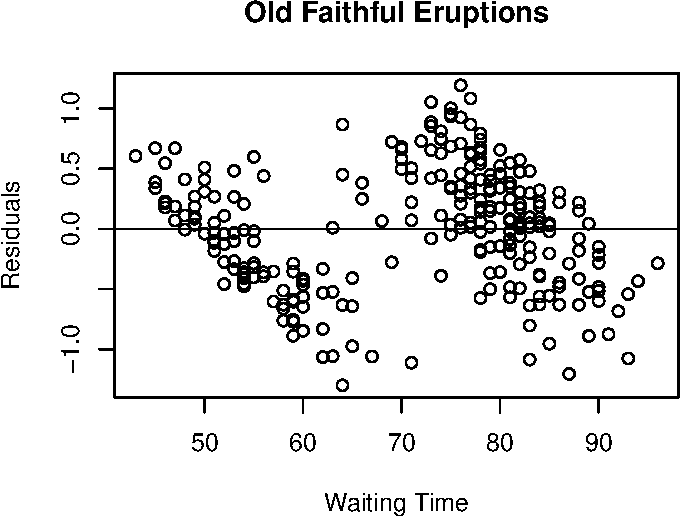
\includegraphics{tema6_files/figure-latex/unnamed-chunk-24-1.pdf}

\subsection{Residuo estandarizado}\label{residuo-estandarizado}

El residuo estandarizado es el residuo dividido por su desviación
estándar.

\[
\mbox{Standardized residual}_i =  \frac{Residual_i}{SD.of.Residual_i}
\]

\begin{Shaded}
\begin{Highlighting}[]
\NormalTok{eruption.stdres <-}\StringTok{ }\KeywordTok{rstandard}\NormalTok{(eruption.lm) }
\end{Highlighting}
\end{Shaded}

\begin{Shaded}
\begin{Highlighting}[]
\KeywordTok{plot}\NormalTok{(faithful$waiting, eruption.stdres, }
      \DataTypeTok{ylab=}\StringTok{"Standardized Residuals"}\NormalTok{, }
      \DataTypeTok{xlab=}\StringTok{"Waiting Time"}\NormalTok{, }
      \DataTypeTok{main=}\StringTok{"Old Faithful Eruptions"}\NormalTok{) }
\KeywordTok{abline}\NormalTok{(}\DecValTok{0}\NormalTok{, }\DecValTok{0}\NormalTok{)}
\end{Highlighting}
\end{Shaded}

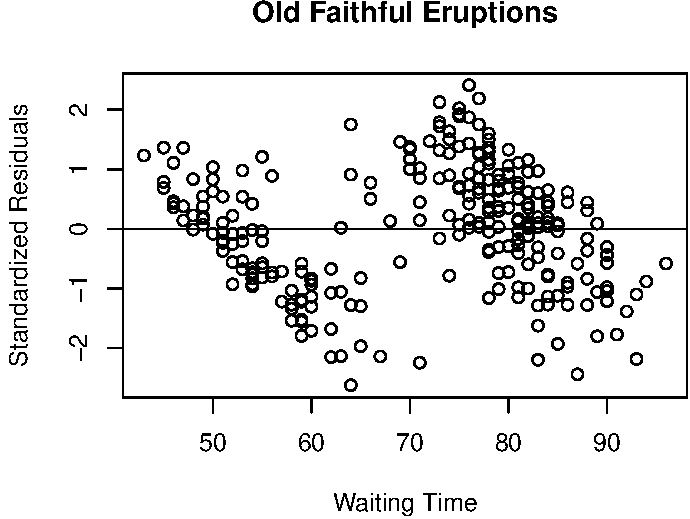
\includegraphics{tema6_files/figure-latex/unnamed-chunk-26-1.pdf}

Como el p-valor es mucho menor que \(0.05\), rechazamos la hipótesis
nula de que \(\beta_1 = 0\). Por lo tanto, existe una relación
significativa entre las variables en el modelo de regresión lineal del
conjunto de datos \texttt{faithful}.

\subsection{Gráfico de normalidad de los
residuos}\label{grafico-de-normalidad-de-los-residuos}

El gráfico de probabilidad normal es una herramienta gráfica para
comparar un conjunto de datos con la distribución normal. Podemos usarlo
con el residuo estandarizado del modelo de regresión lineal y ver si el
término de error \(\epsilon\) es realmente distribuido normalmente.

\begin{Shaded}
\begin{Highlighting}[]
\NormalTok{eruption.lm =}\StringTok{ }\KeywordTok{lm}\NormalTok{(eruptions ~}\StringTok{ }\NormalTok{waiting, }\DataTypeTok{data=}\NormalTok{faithful) }
\NormalTok{eruption.stdres =}\StringTok{ }\KeywordTok{rstandard}\NormalTok{(eruption.lm) }
\end{Highlighting}
\end{Shaded}

Ahora creamos el gráfico de probabilidad normal con la función
\texttt{qqnorm} y añadimos\texttt{qqline} para una comparación
posterior.

\begin{Shaded}
\begin{Highlighting}[]
 \KeywordTok{qqnorm}\NormalTok{(eruption.stdres, }
     \DataTypeTok{ylab=}\StringTok{"Standardized Residuals"}\NormalTok{, }
     \DataTypeTok{xlab=}\StringTok{"Normal Scores"}\NormalTok{, }
     \DataTypeTok{main=}\StringTok{"Old Faithful Eruptions"}\NormalTok{) }
 \KeywordTok{qqline}\NormalTok{(eruption.stdres) }
\end{Highlighting}
\end{Shaded}

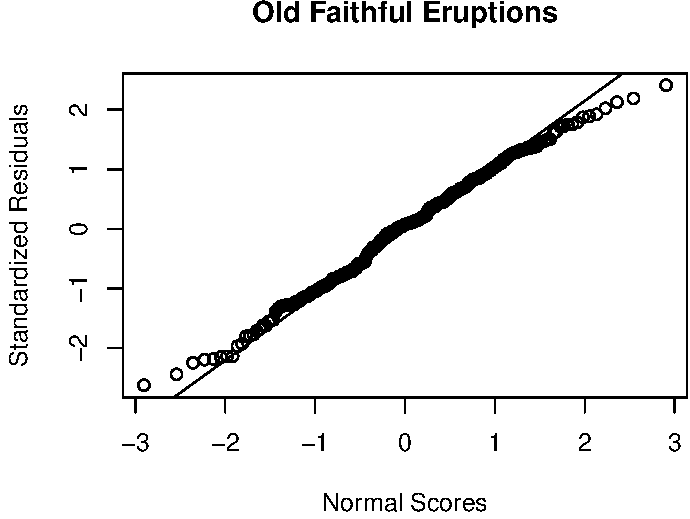
\includegraphics{tema6_files/figure-latex/unnamed-chunk-28-1.pdf}

\subsection{Regresión lineal múltiple}\label{regresion-lineal-multiple}

Un modelo de regresión lineal múltiple describe una variable dependiente
\(y\) por variables independientes \(x_1, x_2, ..., x_p\) \((p> 1)\) se
expresa mediante la ecuación:

\[
    y  = \beta_0 + \sum_{k}^{p} \beta_k + \epsilon
\] donde \(\beta_0\) y \(\beta_k\) (\(k = 1, 2, ..., p\)) son los
parámetros y \(\epsilon\) el término de error.

\textbf{Example:}

Consideremos los datos \texttt{stackloss}, sea \texttt{stackloss} la
variable dependiente, y\texttt{Air.Flow} (cooling air flow),
\texttt{Water.Temp} (inlet water temperature) y \texttt{Acid.Conc.}
(acid concentration) las variables independientes, la regresión multiple
es:

\[
      stack.loss = \beta_0 + \beta_1 * Air.Flow + \beta_2 * Water.Temp + \beta_3 * Acid.Conc + \epsilon
\]

\begin{Shaded}
\begin{Highlighting}[]
\KeywordTok{data}\NormalTok{(}\StringTok{"stackloss"}\NormalTok{)}
\NormalTok{?stackloss}
\KeywordTok{head}\NormalTok{(stackloss)}
\end{Highlighting}
\end{Shaded}

\begin{verbatim}
##   Air.Flow Water.Temp Acid.Conc. stack.loss
## 1       80         27         89         42
## 2       80         27         88         37
## 3       75         25         90         37
## 4       62         24         87         28
## 5       62         22         87         18
## 6       62         23         87         18
\end{verbatim}

El modelo de regresión multiple es:

\begin{Shaded}
\begin{Highlighting}[]
\NormalTok{stackloss.lm =}\StringTok{ }\KeywordTok{lm}\NormalTok{(stack.loss ~}\StringTok{ }\NormalTok{Air.Flow +}\StringTok{ }\NormalTok{Water.Temp +}\StringTok{ }\NormalTok{Acid.Conc., }\DataTypeTok{data=}\NormalTok{stackloss) }
\NormalTok{stackloss.lm}
\end{Highlighting}
\end{Shaded}

\begin{verbatim}
## 
## Call:
## lm(formula = stack.loss ~ Air.Flow + Water.Temp + Acid.Conc., 
##     data = stackloss)
## 
## Coefficients:
## (Intercept)     Air.Flow   Water.Temp   Acid.Conc.  
##    -39.9197       0.7156       1.2953      -0.1521
\end{verbatim}

\begin{Shaded}
\begin{Highlighting}[]
\KeywordTok{summary}\NormalTok{(stackloss.lm)}
\end{Highlighting}
\end{Shaded}

\begin{verbatim}
## 
## Call:
## lm(formula = stack.loss ~ Air.Flow + Water.Temp + Acid.Conc., 
##     data = stackloss)
## 
## Residuals:
##     Min      1Q  Median      3Q     Max 
## -7.2377 -1.7117 -0.4551  2.3614  5.6978 
## 
## Coefficients:
##             Estimate Std. Error t value Pr(>|t|)    
## (Intercept) -39.9197    11.8960  -3.356  0.00375 ** 
## Air.Flow      0.7156     0.1349   5.307  5.8e-05 ***
## Water.Temp    1.2953     0.3680   3.520  0.00263 ** 
## Acid.Conc.   -0.1521     0.1563  -0.973  0.34405    
## ---
## Signif. codes:  0 '***' 0.001 '**' 0.01 '*' 0.05 '.' 0.1 ' ' 1
## 
## Residual standard error: 3.243 on 17 degrees of freedom
## Multiple R-squared:  0.9136, Adjusted R-squared:  0.8983 
## F-statistic:  59.9 on 3 and 17 DF,  p-value: 3.016e-09
\end{verbatim}

La función \texttt{termplot} permite representar los términos de la
regresión frente a las variables predictoras:

\begin{Shaded}
\begin{Highlighting}[]
\NormalTok{?termplot}
\KeywordTok{par}\NormalTok{(}\DataTypeTok{mfrow=}\KeywordTok{c}\NormalTok{(}\DecValTok{2}\NormalTok{,}\DecValTok{2}\NormalTok{))}
\KeywordTok{termplot}\NormalTok{(stackloss.lm, }\DataTypeTok{partial.resid =} \OtherTok{TRUE}\NormalTok{, }\DataTypeTok{se=}\OtherTok{TRUE}\NormalTok{,}\DataTypeTok{col.se =} \StringTok{"blue"}\NormalTok{)}
\end{Highlighting}
\end{Shaded}

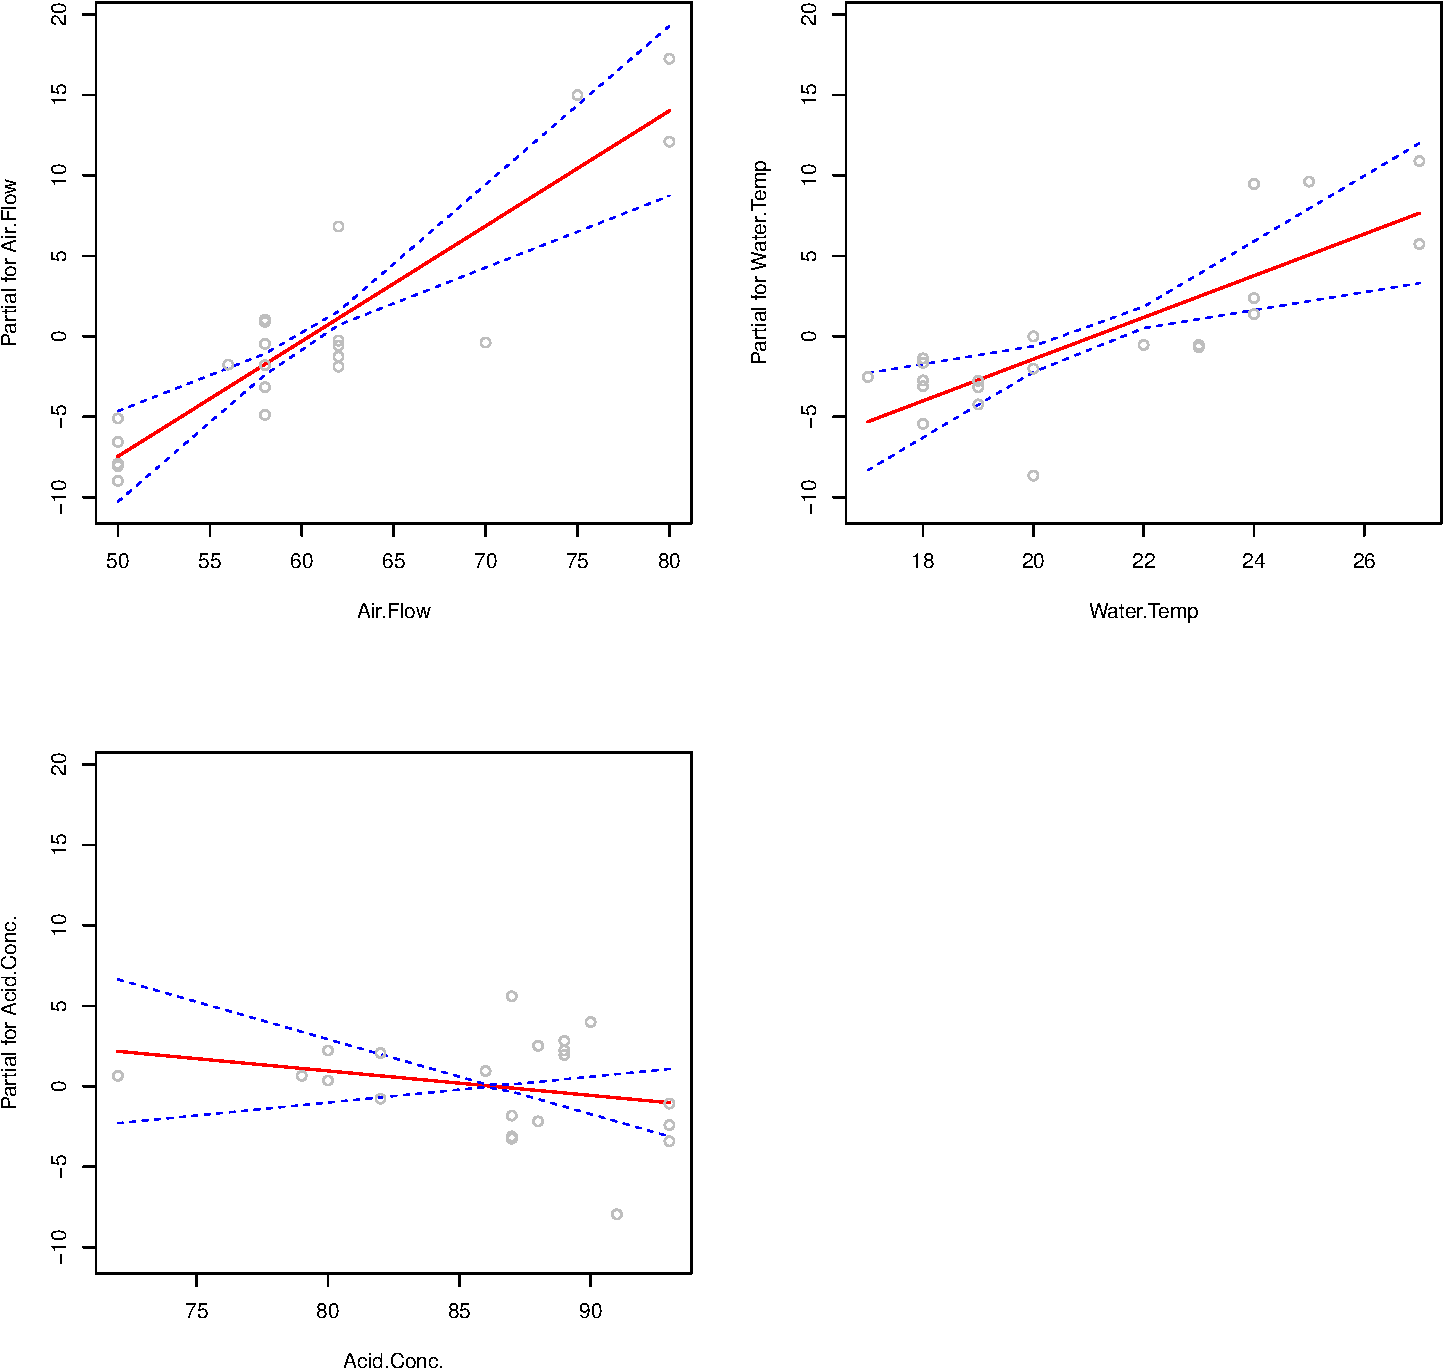
\includegraphics{tema6_files/figure-latex/unnamed-chunk-31-1.pdf}

\textbf{What is the stack loss if the air flow is 72, water temperature
is 20 and acid concentration is 85?}

Crear un nuevo \texttt{data.frame}:

\begin{Shaded}
\begin{Highlighting}[]
\NormalTok{newdata <-}\StringTok{ }\KeywordTok{data.frame}\NormalTok{(}\DataTypeTok{Air.Flow=}\DecValTok{72}\NormalTok{,}\DataTypeTok{Water.Temp=}\DecValTok{20}\NormalTok{,}\DataTypeTok{Acid.Conc.=}\DecValTok{85}\NormalTok{)}
\end{Highlighting}
\end{Shaded}

Con \texttt{predict}

\begin{Shaded}
\begin{Highlighting}[]
\KeywordTok{predict}\NormalTok{(stackloss.lm, newdata) }
\end{Highlighting}
\end{Shaded}

\begin{verbatim}
##        1 
## 24.58173
\end{verbatim}

Basado en el modelo de regresión lineal múltiple y los parámetros dados,
la pérdida prevista es 24.5817284.

Para obtener el coeficiente de determinación múltiple

\begin{Shaded}
\begin{Highlighting}[]
\KeywordTok{summary}\NormalTok{(stackloss.lm)$r.squared }
\end{Highlighting}
\end{Shaded}

\begin{verbatim}
## [1] 0.9135769
\end{verbatim}

\subsubsection{Coeficiente de determinación
ajustado}\label{coeficiente-de-determinacion-ajustado}

El coeficiente de determinación ajustado de un modelo de regresión
lineal múltiple se define en términos del coeficiente de determinación
como sigue, donde \(n\) es el número de observaciones en el conjunto de
datos y \(p\) es el número de variables independientes.

\[
R^2_{adj} = 1-(1-R^2)\frac{n-1}{n-p-1}
\]

\begin{Shaded}
\begin{Highlighting}[]
\KeywordTok{summary}\NormalTok{(stackloss.lm)$adj.r.squared }
\end{Highlighting}
\end{Shaded}

\begin{verbatim}
## [1] 0.8983258
\end{verbatim}

\subsubsection{Pruebas de significación e intervalos de confianza /
predicción}\label{pruebas-de-significacion-e-intervalos-de-confianza-prediccion}

\begin{Shaded}
\begin{Highlighting}[]
\KeywordTok{summary}\NormalTok{(stackloss.lm)}
\end{Highlighting}
\end{Shaded}

\begin{verbatim}
## 
## Call:
## lm(formula = stack.loss ~ Air.Flow + Water.Temp + Acid.Conc., 
##     data = stackloss)
## 
## Residuals:
##     Min      1Q  Median      3Q     Max 
## -7.2377 -1.7117 -0.4551  2.3614  5.6978 
## 
## Coefficients:
##             Estimate Std. Error t value Pr(>|t|)    
## (Intercept) -39.9197    11.8960  -3.356  0.00375 ** 
## Air.Flow      0.7156     0.1349   5.307  5.8e-05 ***
## Water.Temp    1.2953     0.3680   3.520  0.00263 ** 
## Acid.Conc.   -0.1521     0.1563  -0.973  0.34405    
## ---
## Signif. codes:  0 '***' 0.001 '**' 0.01 '*' 0.05 '.' 0.1 ' ' 1
## 
## Residual standard error: 3.243 on 17 degrees of freedom
## Multiple R-squared:  0.9136, Adjusted R-squared:  0.8983 
## F-statistic:  59.9 on 3 and 17 DF,  p-value: 3.016e-09
\end{verbatim}

Como los p-valores de \texttt{Air.Flow} y\texttt{Water.Temp} son
inferiores a 0,05, ambos son estadísticamente significativos en el
modelo de regresión lineal múltiple de \texttt{stackloss}.

El intervalo de confianza al 95\% de \texttt{stackloss} es

\begin{Shaded}
\begin{Highlighting}[]
\KeywordTok{predict}\NormalTok{(stackloss.lm, newdata, }\DataTypeTok{interval=}\StringTok{"confidence"}\NormalTok{)}
\end{Highlighting}
\end{Shaded}

\begin{verbatim}
##        fit      lwr    upr
## 1 24.58173 20.21846 28.945
\end{verbatim}

Y el invervalo de predicción al 95\%

\begin{Shaded}
\begin{Highlighting}[]
\KeywordTok{predict}\NormalTok{(stackloss.lm, newdata, }\DataTypeTok{interval=}\StringTok{"prediction"}\NormalTok{)}
\end{Highlighting}
\end{Shaded}

\begin{verbatim}
##        fit     lwr      upr
## 1 24.58173 16.4661 32.69736
\end{verbatim}

\subsection{Regresión lineal con variables
factor}\label{regresion-lineal-con-variables-factor}

Supongamos el conjunto de datos \texttt{mtcars}.

\begin{Shaded}
\begin{Highlighting}[]
\KeywordTok{data}\NormalTok{(mtcars)}
\KeywordTok{t.test}\NormalTok{(mpg ~}\StringTok{ }\NormalTok{am, }\DataTypeTok{data=}\NormalTok{mtcars) }
\end{Highlighting}
\end{Shaded}

\begin{verbatim}
## 
##  Welch Two Sample t-test
## 
## data:  mpg by am
## t = -3.7671, df = 18.332, p-value = 0.001374
## alternative hypothesis: true difference in means is not equal to 0
## 95 percent confidence interval:
##  -11.280194  -3.209684
## sample estimates:
## mean in group 0 mean in group 1 
##        17.14737        24.39231
\end{verbatim}

Los resultados de las pruebas estadísticas se centran en \texttt{mpg}
y\texttt{am} solamente, sin controlar las influencias de otras
variables.

\begin{Shaded}
\begin{Highlighting}[]
\NormalTok{fit0 <-}\StringTok{ }\KeywordTok{lm}\NormalTok{(mpg ~}\StringTok{ }\KeywordTok{factor}\NormalTok{(am), }\DataTypeTok{data =} \NormalTok{mtcars)}
\KeywordTok{summary}\NormalTok{(fit0)}
\end{Highlighting}
\end{Shaded}

\begin{verbatim}
## 
## Call:
## lm(formula = mpg ~ factor(am), data = mtcars)
## 
## Residuals:
##     Min      1Q  Median      3Q     Max 
## -9.3923 -3.0923 -0.2974  3.2439  9.5077 
## 
## Coefficients:
##             Estimate Std. Error t value Pr(>|t|)    
## (Intercept)   17.147      1.125  15.247 1.13e-15 ***
## factor(am)1    7.245      1.764   4.106 0.000285 ***
## ---
## Signif. codes:  0 '***' 0.001 '**' 0.01 '*' 0.05 '.' 0.1 ' ' 1
## 
## Residual standard error: 4.902 on 30 degrees of freedom
## Multiple R-squared:  0.3598, Adjusted R-squared:  0.3385 
## F-statistic: 16.86 on 1 and 30 DF,  p-value: 0.000285
\end{verbatim}

Si aplicamos una regresión multiple para controlar ciertas variables
disponibles de diseño y rendimiento, el impacto marginal de los
automóviles de transmisión automática o manual no resulta significativo.
Las variables de confusión incluyen desplazamiento (\texttt{disp}),
relación del eje trasero (\texttt{drat}) y peso del coche (\texttt{wt}).
Supongamos el peso del coche (\texttt{wt}) por ejemplo. La regresión
sugiere que, manteniendo constantes otras variables (ceteris paribus),
los automóviles traídos por tracción consumen -0.024 galones más de gas
por milla y los resultados ya no son estadísticamente significativos. Un
análisis similar se puede observar para las otras dos variables:
\texttt{drat} y \texttt{wt}.

\begin{Shaded}
\begin{Highlighting}[]
\NormalTok{fit1 <-}\StringTok{ }\KeywordTok{lm}\NormalTok{(mpg ~}\StringTok{ }\KeywordTok{factor}\NormalTok{(am) +}\StringTok{ }\NormalTok{wt, }\DataTypeTok{data =} \NormalTok{mtcars)}
\KeywordTok{summary}\NormalTok{(fit1)}
\end{Highlighting}
\end{Shaded}

\begin{verbatim}
## 
## Call:
## lm(formula = mpg ~ factor(am) + wt, data = mtcars)
## 
## Residuals:
##     Min      1Q  Median      3Q     Max 
## -4.5295 -2.3619 -0.1317  1.4025  6.8782 
## 
## Coefficients:
##             Estimate Std. Error t value Pr(>|t|)    
## (Intercept) 37.32155    3.05464  12.218 5.84e-13 ***
## factor(am)1 -0.02362    1.54565  -0.015    0.988    
## wt          -5.35281    0.78824  -6.791 1.87e-07 ***
## ---
## Signif. codes:  0 '***' 0.001 '**' 0.01 '*' 0.05 '.' 0.1 ' ' 1
## 
## Residual standard error: 3.098 on 29 degrees of freedom
## Multiple R-squared:  0.7528, Adjusted R-squared:  0.7358 
## F-statistic: 44.17 on 2 and 29 DF,  p-value: 1.579e-09
\end{verbatim}

\begin{Shaded}
\begin{Highlighting}[]
\NormalTok{fit2 <-}\StringTok{ }\KeywordTok{lm}\NormalTok{(mpg ~}\StringTok{ }\KeywordTok{factor}\NormalTok{(am) +}\StringTok{ }\NormalTok{drat, }\DataTypeTok{data =} \NormalTok{mtcars)}
\KeywordTok{summary}\NormalTok{(fit2)}
\end{Highlighting}
\end{Shaded}

\begin{verbatim}
## 
## Call:
## lm(formula = mpg ~ factor(am) + drat, data = mtcars)
## 
## Residuals:
##     Min      1Q  Median      3Q     Max 
## -9.5802 -2.5206 -0.5153  2.4419  8.5198 
## 
## Coefficients:
##             Estimate Std. Error t value Pr(>|t|)  
## (Intercept)   -1.950      7.073  -0.276   0.7848  
## factor(am)1    2.807      2.282   1.230   0.2286  
## drat           5.811      2.130   2.728   0.0107 *
## ---
## Signif. codes:  0 '***' 0.001 '**' 0.01 '*' 0.05 '.' 0.1 ' ' 1
## 
## Residual standard error: 4.448 on 29 degrees of freedom
## Multiple R-squared:  0.4906, Adjusted R-squared:  0.4554 
## F-statistic: 13.96 on 2 and 29 DF,  p-value: 5.659e-05
\end{verbatim}

\begin{Shaded}
\begin{Highlighting}[]
\NormalTok{fit3 <-}\StringTok{ }\KeywordTok{lm}\NormalTok{(mpg ~}\StringTok{ }\KeywordTok{factor}\NormalTok{(am) +}\StringTok{ }\NormalTok{disp, }\DataTypeTok{data =} \NormalTok{mtcars)}
\KeywordTok{summary}\NormalTok{(fit3)}
\end{Highlighting}
\end{Shaded}

\begin{verbatim}
## 
## Call:
## lm(formula = mpg ~ factor(am) + disp, data = mtcars)
## 
## Residuals:
##     Min      1Q  Median      3Q     Max 
## -4.6382 -2.4751 -0.5631  2.2333  6.8386 
## 
## Coefficients:
##              Estimate Std. Error t value Pr(>|t|)    
## (Intercept) 27.848081   1.834071  15.184 2.45e-15 ***
## factor(am)1  1.833458   1.436100   1.277    0.212    
## disp        -0.036851   0.005782  -6.373 5.75e-07 ***
## ---
## Signif. codes:  0 '***' 0.001 '**' 0.01 '*' 0.05 '.' 0.1 ' ' 1
## 
## Residual standard error: 3.218 on 29 degrees of freedom
## Multiple R-squared:  0.7333, Adjusted R-squared:  0.7149 
## F-statistic: 39.87 on 2 and 29 DF,  p-value: 4.749e-09
\end{verbatim}

Con \texttt{termplot}

\begin{Shaded}
\begin{Highlighting}[]
\KeywordTok{termplot}\NormalTok{(fit0,}\DataTypeTok{partial.resid =} \OtherTok{TRUE}\NormalTok{,}\DataTypeTok{se=}\OtherTok{TRUE}\NormalTok{)}
\end{Highlighting}
\end{Shaded}

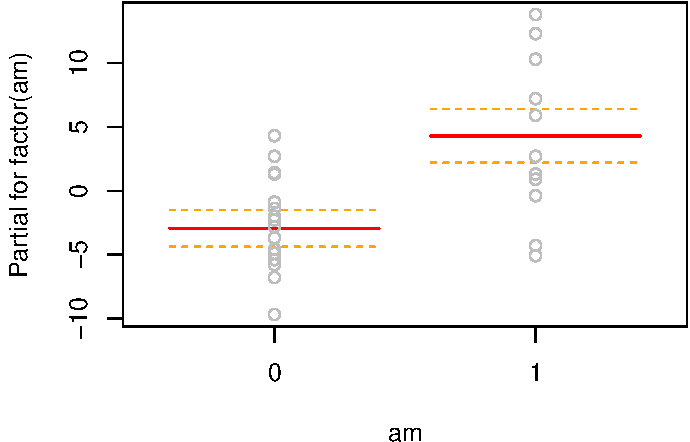
\includegraphics{tema6_files/figure-latex/unnamed-chunk-43-1.pdf}

\begin{Shaded}
\begin{Highlighting}[]
\KeywordTok{par}\NormalTok{(}\DataTypeTok{mfrow=}\KeywordTok{c}\NormalTok{(}\DecValTok{1}\NormalTok{,}\DecValTok{2}\NormalTok{))}
\KeywordTok{termplot}\NormalTok{(fit1,}\DataTypeTok{partial.resid =} \OtherTok{TRUE}\NormalTok{,}\DataTypeTok{se=}\OtherTok{TRUE}\NormalTok{)}
\end{Highlighting}
\end{Shaded}

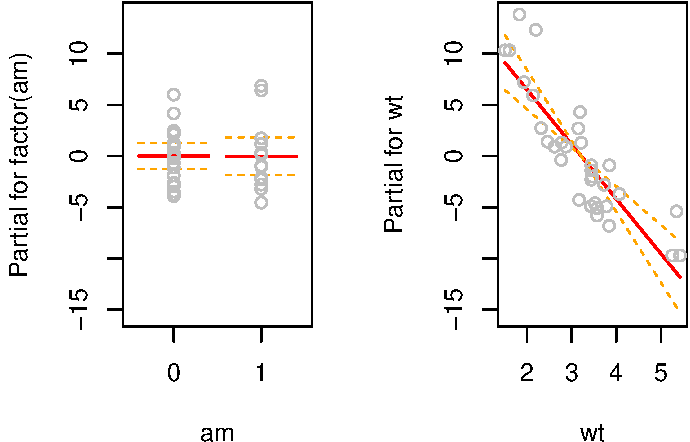
\includegraphics{tema6_files/figure-latex/unnamed-chunk-44-1.pdf}

\begin{Shaded}
\begin{Highlighting}[]
\KeywordTok{termplot}\NormalTok{(fit2,}\DataTypeTok{partial.resid =} \OtherTok{TRUE}\NormalTok{,}\DataTypeTok{se=}\OtherTok{TRUE}\NormalTok{)}
\end{Highlighting}
\end{Shaded}

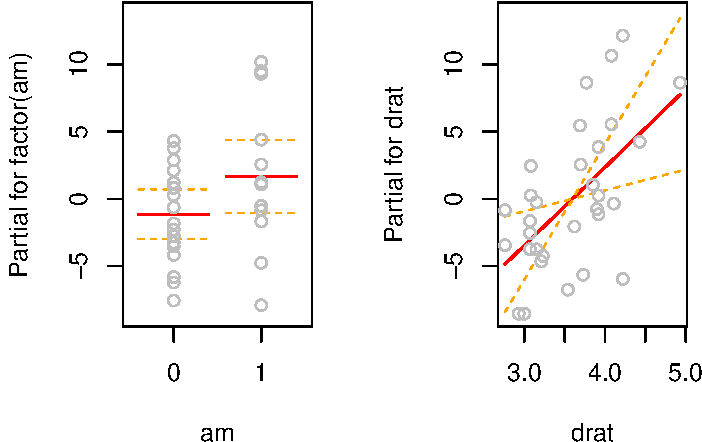
\includegraphics{tema6_files/figure-latex/unnamed-chunk-44-2.pdf}

\subsection{Inferencia de modelos
lineales}\label{inferencia-de-modelos-lineales}

\textbf{Comparación de modelos: test de razón de verosimitudes}

Es una prueba estadística utilizada para comparar la bondad de ajuste de
dos modelos, uno de los cuales (el modelo nulo) es un caso especial del
otro (el modelo alternativo). La prueba se basa en la razón de
verosimilitud, que expresa cuántas veces más probabilidades de que los
datos estén bajo un modelo que el otro.

La comparación de dos modelos ajustados a los mismos datos se puede
configurar como un problema de prueba de hipótesis. Sea \(M_0\) y
\(M_1\) los modelos.

Consideremos como la hipótesis nula \emph{``\$ M\_1 \$ no es una mejora
significativa en \$ M\_0 \$''}, y la alternativa la negación. Esta
hipótesis se puede formular a menudo de modo que un estadístico se pueda
generar de los dos modelos.

Normalmente, los modelos se anidan en que las variables en \(M_0\) son
un subconjunto de los de \(M_1\). La estadística a menudo involucra los
valores \(RSS\) (suma residual de cuadrados) para ambos modelos,
ajustados por el número de parámetros utilizados. En la regresión lineal
esto se convierte en una prueba de \texttt{anova} (comparando las
varianzas).

\begin{Shaded}
\begin{Highlighting}[]
\NormalTok{M0 <-}\StringTok{ }\KeywordTok{lm}\NormalTok{(mpg ~}\StringTok{ }\DecValTok{1}\NormalTok{, }\DataTypeTok{data =} \NormalTok{mtcars)}
\NormalTok{M1 <-}\StringTok{ }\KeywordTok{lm}\NormalTok{(mpg ~}\StringTok{ }\KeywordTok{factor}\NormalTok{(am), }\DataTypeTok{data =} \NormalTok{mtcars)}
\KeywordTok{summary}\NormalTok{(M0)}
\end{Highlighting}
\end{Shaded}

\begin{verbatim}
## 
## Call:
## lm(formula = mpg ~ 1, data = mtcars)
## 
## Residuals:
##     Min      1Q  Median      3Q     Max 
## -9.6906 -4.6656 -0.8906  2.7094 13.8094 
## 
## Coefficients:
##             Estimate Std. Error t value Pr(>|t|)    
## (Intercept)   20.091      1.065   18.86   <2e-16 ***
## ---
## Signif. codes:  0 '***' 0.001 '**' 0.01 '*' 0.05 '.' 0.1 ' ' 1
## 
## Residual standard error: 6.027 on 31 degrees of freedom
\end{verbatim}

\begin{Shaded}
\begin{Highlighting}[]
\KeywordTok{summary}\NormalTok{(M1)}
\end{Highlighting}
\end{Shaded}

\begin{verbatim}
## 
## Call:
## lm(formula = mpg ~ factor(am), data = mtcars)
## 
## Residuals:
##     Min      1Q  Median      3Q     Max 
## -9.3923 -3.0923 -0.2974  3.2439  9.5077 
## 
## Coefficients:
##             Estimate Std. Error t value Pr(>|t|)    
## (Intercept)   17.147      1.125  15.247 1.13e-15 ***
## factor(am)1    7.245      1.764   4.106 0.000285 ***
## ---
## Signif. codes:  0 '***' 0.001 '**' 0.01 '*' 0.05 '.' 0.1 ' ' 1
## 
## Residual standard error: 4.902 on 30 degrees of freedom
## Multiple R-squared:  0.3598, Adjusted R-squared:  0.3385 
## F-statistic: 16.86 on 1 and 30 DF,  p-value: 0.000285
\end{verbatim}

\begin{Shaded}
\begin{Highlighting}[]
\KeywordTok{anova}\NormalTok{(M0,M1)}
\end{Highlighting}
\end{Shaded}

\begin{verbatim}
## Analysis of Variance Table
## 
## Model 1: mpg ~ 1
## Model 2: mpg ~ factor(am)
##   Res.Df    RSS Df Sum of Sq     F   Pr(>F)    
## 1     31 1126.0                                
## 2     30  720.9  1    405.15 16.86 0.000285 ***
## ---
## Signif. codes:  0 '***' 0.001 '**' 0.01 '*' 0.05 '.' 0.1 ' ' 1
\end{verbatim}

La prueba/test de razón de verosimilitud también puede probar la
significación de los predictores. Por lo tanto, podemos comparar el
modelo \texttt{fit0} (donde\texttt{am} es significativo) con
\texttt{fit1},\texttt{fit2} o \texttt{fit3}, es decir:

\begin{Shaded}
\begin{Highlighting}[]
\KeywordTok{anova}\NormalTok{(fit0, fit1)}
\end{Highlighting}
\end{Shaded}

\begin{verbatim}
## Analysis of Variance Table
## 
## Model 1: mpg ~ factor(am)
## Model 2: mpg ~ factor(am) + wt
##   Res.Df    RSS Df Sum of Sq      F    Pr(>F)    
## 1     30 720.90                                  
## 2     29 278.32  1    442.58 46.115 1.867e-07 ***
## ---
## Signif. codes:  0 '***' 0.001 '**' 0.01 '*' 0.05 '.' 0.1 ' ' 1
\end{verbatim}

\begin{Shaded}
\begin{Highlighting}[]
\KeywordTok{anova}\NormalTok{(fit0, fit2)}
\end{Highlighting}
\end{Shaded}

\begin{verbatim}
## Analysis of Variance Table
## 
## Model 1: mpg ~ factor(am)
## Model 2: mpg ~ factor(am) + drat
##   Res.Df    RSS Df Sum of Sq      F Pr(>F)  
## 1     30 720.90                             
## 2     29 573.64  1    147.26 7.4444 0.0107 *
## ---
## Signif. codes:  0 '***' 0.001 '**' 0.01 '*' 0.05 '.' 0.1 ' ' 1
\end{verbatim}

\begin{Shaded}
\begin{Highlighting}[]
\KeywordTok{anova}\NormalTok{(fit0, fit3)}
\end{Highlighting}
\end{Shaded}

\begin{verbatim}
## Analysis of Variance Table
## 
## Model 1: mpg ~ factor(am)
## Model 2: mpg ~ factor(am) + disp
##   Res.Df    RSS Df Sum of Sq      F    Pr(>F)    
## 1     30 720.90                                  
## 2     29 300.28  1    420.62 40.621 5.748e-07 ***
## ---
## Signif. codes:  0 '***' 0.001 '**' 0.01 '*' 0.05 '.' 0.1 ' ' 1
\end{verbatim}

Sin embargo, las pruebas de razón de verosimilitud sugieren que es
importante considerar estas dimensiones (es decir, el desplazamiento, la
relación del eje trasero y el peso) ya que estas variables aumentan el
ajuste del modelo.

\begin{Shaded}
\begin{Highlighting}[]
\KeywordTok{library}\NormalTok{(faraway)}
\KeywordTok{data}\NormalTok{(pima, }\DataTypeTok{package=}\StringTok{"faraway"}\NormalTok{)}
\KeywordTok{head}\NormalTok{(pima)}
\KeywordTok{summary}\NormalTok{(pima)}
\KeywordTok{sort}\NormalTok{(pima$diastolic)}
\NormalTok{pima$diastolic[pima$diastolic ==}\StringTok{ }\DecValTok{0}\NormalTok{]  <-}\StringTok{ }\OtherTok{NA}
\NormalTok{pima$glucose[pima$glucose ==}\StringTok{ }\DecValTok{0}\NormalTok{] <-}\StringTok{ }\OtherTok{NA}
\NormalTok{pima$triceps[pima$triceps ==}\StringTok{ }\DecValTok{0}\NormalTok{]  <-}\StringTok{ }\OtherTok{NA}
\NormalTok{pima$insulin[pima$insulin ==}\StringTok{ }\DecValTok{0}\NormalTok{] <-}\StringTok{ }\OtherTok{NA}
\NormalTok{pima$bmi[pima$bmi ==}\StringTok{ }\DecValTok{0}\NormalTok{] <-}\StringTok{ }\OtherTok{NA}
\NormalTok{pima$test <-}\StringTok{ }\KeywordTok{factor}\NormalTok{(pima$test)}
\KeywordTok{summary}\NormalTok{(pima$test)}
\KeywordTok{levels}\NormalTok{(pima$test) <-}\StringTok{ }\KeywordTok{c}\NormalTok{(}\StringTok{"negative"}\NormalTok{,}\StringTok{"positive"}\NormalTok{)}
\KeywordTok{summary}\NormalTok{(pima)}
\KeywordTok{hist}\NormalTok{(pima$diastolic,}\DataTypeTok{xlab=}\StringTok{"Diastolic"}\NormalTok{,}\DataTypeTok{main=}\StringTok{""}\NormalTok{)}
\KeywordTok{plot}\NormalTok{(}\KeywordTok{density}\NormalTok{(pima$diastolic,}\DataTypeTok{na.rm=}\OtherTok{TRUE}\NormalTok{),}\DataTypeTok{main=}\StringTok{""}\NormalTok{)}
\KeywordTok{plot}\NormalTok{(}\KeywordTok{sort}\NormalTok{(pima$diastolic),}\DataTypeTok{ylab=}\StringTok{"Sorted Diastolic"}\NormalTok{)}
\KeywordTok{plot}\NormalTok{(diabetes ~}\StringTok{ }\NormalTok{diastolic,pima)}
\KeywordTok{plot}\NormalTok{(diabetes ~}\StringTok{ }\NormalTok{test,pima)}
\KeywordTok{require}\NormalTok{(ggplot2)}
\KeywordTok{ggplot}\NormalTok{(pima,}\KeywordTok{aes}\NormalTok{(}\DataTypeTok{x=}\NormalTok{diastolic))+}\KeywordTok{geom_histogram}\NormalTok{()}
\KeywordTok{ggplot}\NormalTok{(pima,}\KeywordTok{aes}\NormalTok{(}\DataTypeTok{x=}\NormalTok{diastolic))+}\KeywordTok{geom_density}\NormalTok{()}
\KeywordTok{ggplot}\NormalTok{(pima,}\KeywordTok{aes}\NormalTok{(}\DataTypeTok{x=}\NormalTok{diastolic,}\DataTypeTok{y=}\NormalTok{diabetes))+}\KeywordTok{geom_point}\NormalTok{()}
\KeywordTok{ggplot}\NormalTok{(pima,}\KeywordTok{aes}\NormalTok{(}\DataTypeTok{x=}\NormalTok{diastolic,}\DataTypeTok{y=}\NormalTok{diabetes,}\DataTypeTok{shape=}\NormalTok{test))+}\KeywordTok{geom_point}\NormalTok{()+}\KeywordTok{theme}\NormalTok{(}\DataTypeTok{legend.position =} \StringTok{"top"}\NormalTok{, }\DataTypeTok{legend.direction =} \StringTok{"horizontal"}\NormalTok{)}
\KeywordTok{ggplot}\NormalTok{(pima,}\KeywordTok{aes}\NormalTok{(}\DataTypeTok{x=}\NormalTok{diastolic,}\DataTypeTok{y=}\NormalTok{diabetes)) +}\StringTok{ }\KeywordTok{geom_point}\NormalTok{(}\DataTypeTok{size=}\DecValTok{1}\NormalTok{) +}\StringTok{ }\KeywordTok{facet_grid}\NormalTok{(~}\StringTok{ }\NormalTok{test)}
\end{Highlighting}
\end{Shaded}

\end{document}